\section{测度的构造}
\label{sec:meas-construction}

上一节规定了测度应满足的规则，并用计数、点质量等例子验证了这些规则可以实现。可是第~\ref{sec:meas-size-additivity}节真正想要的长度测度还没有出现：我们只知道区间的长度，并不知道怎样把它可数可加地推广到$\mathcal B(\mathbb R)$。

本节分三步回答。先把可数覆盖的想法做成外测度，从中选出满足分割可加的集合；再把这条路线抽象成从简单集合族出发的延拓定理，分别回答延拓是否存在、是否唯一；最后用它构造实轴上的Lebesgue测度和Stieltjes测度。

\subsection{外测度}
\label{sec:meas-outer-measure}

\paragraph{覆盖的总费用}
有理点集的例子提示了一种测量方式：用一列简单集合覆盖待测集合，算出覆盖的总费用，再让总费用尽量小。可以把简单集合想成一种按件定价的“包装”，给一个集合算大小，就是问把它完全打包最少要花多少钱。这样得到的量对每个子集都有定义，但它满足的规则比测度少。

\begin{definition}[外测度]
\label{def:meas-outer}
集合$X$上的\term{外测度}（outer measure）是映射$\mu^*:\mathcal P(X)\to[0,+\infty]$，满足：$\mu^*(\varnothing)=0$；$E\subseteq F$蕴含$\mu^*(E)\leq\mu^*(F)$；对任意$E_1,E_2,\dots\subseteq X$，有
\begin{equation}
 \mu^*\Bigl(\bigcup_nE_n\Bigr)\leq\sum_n\mu^*(E_n).
 \label{eq:meas-outer-subadditive}
\end{equation}
\end{definition}

外测度只要求次可加，不要求可加。下面的引理说明，任何一种“简单集合的费用”都能经可数覆盖变成外测度，这就是把局部赋值推广到任意子集的方法。

\begin{lemma}[由覆盖得到外测度]
\label{lem:meas-cover-outer}
设$\mathcal C$是$X$的一族子集，$\varnothing\in\mathcal C$，$\rho:\mathcal C\to[0,+\infty]$满足$\rho(\varnothing)=0$。对$E\subseteq X$令
\begin{equation}
 \mu^*(E)=\inf\Bigl\{\sum_{n\geq1}\rho(C_n):C_n\in\mathcal C,\ E\subseteq\bigcup_{n\geq1}C_n\Bigr\},
 \label{eq:meas-cover-outer}
\end{equation}
没有这样的覆盖时取$+\infty$。则$\mu^*$是外测度。
\end{lemma}

\begin{proof}
取全部$C_n=\varnothing$覆盖空集，得$\mu^*(\varnothing)=0$。若$E\subseteq F$，覆盖$F$的每一列集合也覆盖$E$，下确界取在更大的范围上，故$\mu^*(E)\leq\mu^*(F)$。

对次可加性，不妨设$\sum_n\mu^*(E_n)<+\infty$，任取$\varepsilon>0$。对每个$n$，按下确界的定义选覆盖$E_n$的$C_{n,1},C_{n,2},\dots\in\mathcal C$，使
\[
 \sum_k\rho(C_{n,k})\leq\mu^*(E_n)+\varepsilon2^{-n}.
\]

全体$C_{n,k}$可以排成一列并覆盖$\bigcup_nE_n$，非负项的排列不改变级数和，于是
\[
 \mu^*\Bigl(\bigcup_nE_n\Bigr)\leq\sum_n\sum_k\rho(C_{n,k})
 \leq\sum_n\bigl(\mu^*(E_n)+\varepsilon2^{-n}\bigr)=\sum_n\mu^*(E_n)+\varepsilon.
\]
令$\varepsilon\to0$即得结论。
\end{proof}

外测度能给每个子集赋值，代价是失去可加性。在$X=\{1,2\}$上取$\mathcal C=\{\varnothing,X\}$、$\rho(X)=1$。唯一有效的覆盖是$X$本身，所以
\[
 \mu^*(\{1\})=\mu^*(\{2\})=\mu^*(X)=1.
\]
不交的$\{1\}$与$\{2\}$外测度之和为$2$，它们的并的外测度却是$1$。原因是这份价目表只卖整包，无法把两点分开计价，见图~\ref{fig:meas-carath-cut}(b)。因此要找出外测度在哪些集合上可加。

\paragraph{Carathéodory可测性}
一个集合$A$要“与外测度相容”，应当意味着用$A$去切任何集合都不会多算或少算。图~\ref{fig:meas-carath-cut}(a)画的正是这个检验：拿一个测试集合$E$，用$A$切成两块，比较切开前后的总价。只在一个特定的$E$上检验还不够，下面的判据要求对一切测试集合都成立。

\begin{BookInlineFigure}
  \centering
  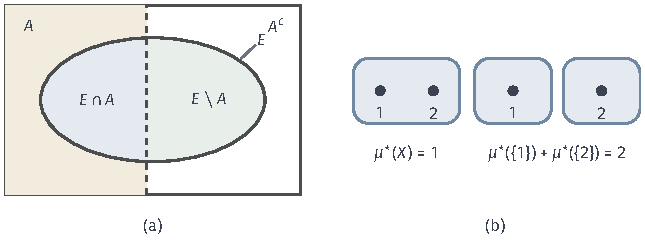
\includegraphics[width=109.238mm]{figures/04-spaces-measures-and-geometry/02-measure/tikz/meas-carath-cut/figure.pdf}
  \caption{Carathéodory判据的含义。(a)测试集合$E$（椭圆）被$A$切成$E\cap A$（蓝）与$E\setminus A$（绿），可测要求两块的外测度之和总等于$\mu^*(E)$；(b)价目表只卖整包$X$时，切开$X=\{1,2\}$迫使每点各付一个整包的价，$\{1\}$不满足判据。}
  \label{fig:meas-carath-cut}
\end{BookInlineFigure}

\begin{definition}[Carathéodory可测]
\label{def:meas-caratheodory-measurable}
设$\mu^*$是$X$上的外测度。若对每个$E\subseteq X$都有
\begin{equation}
 \mu^*(E)=\mu^*(E\cap A)+\mu^*(E\setminus A),
 \label{eq:meas-caratheodory-criterion}
\end{equation}
称$A\subseteq X$为$\mu^*$-\term{Carathéodory可测}（Carathéodory measurable）的。
\end{definition}

由次可加性，“$\leq$”总成立，所以验证时只需证明“$\geq$”，并且只需对$\mu^*(E)<+\infty$的$E$验证。上例中$\{1\}$不满足判据：取$E=X$，右边为$2$，左边为$1$。

再看一个能选出非平凡集合的例子。取$X=\{1,2,3\}$，价目表$\mathcal C=\{\varnothing,\{1\},\{2,3\},X\}$，价格为
\[
 \rho(\{1\})=1,\qquad\rho(\{2,3\})=2,\qquad\rho(X)=3.
\]
点$2$、$3$只能打包购买。由式~\eqref{eq:meas-cover-outer}，单点和两点集的外测度是
\[
 \mu^*(\{1\})=1,\quad \mu^*(\{2\})=\mu^*(\{3\})=\mu^*(\{2,3\})=2,\quad \mu^*(\{1,2\})=3.
\]

检验$A=\{1\}$：取$E=X$，$1+2=3$；取$E=\{2\}$，$0+2=2$；取$E=\{1,2\}$，$1+2=3$，等式都成立，其余$E$同样核对。检验$A=\{2\}$：取$E=\{2,3\}$，右边是$\mu^*(\{2\})+\mu^*(\{3\})=4$，左边是$2$，判据不成立。

逐一检查可知全部可测集是$\varnothing,\{1\},\{2,3\},X$：恰好是价目表上明码标价的那些集合。下面的定理说明，这样选出的集合总是构成$\sigma$代数，外测度在上面可数可加。

\begin{theorem}[Carathéodory定理]
\label{thm:meas-caratheodory}
设$\mu^*$是$X$上的外测度，$\mathcal M$为全体$\mu^*$-Carathéodory可测集。则$\mathcal M$是$\sigma$代数，$\mu^*$在$\mathcal M$上的限制是测度，且$(X,\mathcal M,\mu^*|_{\mathcal M})$完备；特别地，$\mu^*(N)=0$的集合$N$都属于$\mathcal M$。
\end{theorem}

证明分三步：先处理补集与有限并，再控制可数不交并，最后由不交化得到一般的可数并，同时读出可数可加性。

\begin{proof}
\emph{补集与有限并。}判据关于$A$与$X\setminus A$对称，所以$\mathcal M$对补集封闭；$X\in\mathcal M$是因为$\mu^*(\varnothing)=0$。

设$A,B\in\mathcal M$，$E\subseteq X$。先用$A$切$E$，再用$B$切$E\setminus A$，得到
\[
 \mu^*(E)=\mu^*(E\cap A)+\mu^*\bigl((E\setminus A)\cap B\bigr)+\mu^*\bigl(E\setminus(A\cup B)\bigr).
\]
把前两项涉及的两块并起来，就是$A\cup B$切出的部分：
\[
 E\cap(A\cup B)=(E\cap A)\cup\bigl((E\setminus A)\cap B\bigr).
\]
次可加性说明前两项之和不小于$\mu^*(E\cap(A\cup B))$，于是
\[
 \mu^*(E)\geq\mu^*\bigl(E\cap(A\cup B)\bigr)+\mu^*\bigl(E\setminus(A\cup B)\bigr).
\]
这就是$A\cup B$的判据。于是$\mathcal M$对有限并、有限交与差都封闭。

\emph{可数不交并。}设$A_1,A_2,\dots\in\mathcal M$两两不交，$B_n=\bigcup_{k\leq n}A_k$，$B=\bigcup_kA_k$。用$A_n$切测试集合$E\cap B_n$，因$A_n$与$B_{n-1}$不交，得
\[
 \mu^*(E\cap B_n)=\mu^*(E\cap A_n)+\mu^*(E\cap B_{n-1}).
\]
对$n$归纳，得到
\[
 \mu^*(E\cap B_n)=\sum_{k\leq n}\mu^*(E\cap A_k).
\]

再用$B_n\in\mathcal M$切$E$，并由$E\setminus B_n\supseteq E\setminus B$及单调性，得
\[
 \mu^*(E)=\mu^*(E\cap B_n)+\mu^*(E\setminus B_n)
 \geq\sum_{k\leq n}\mu^*(E\cap A_k)+\mu^*(E\setminus B).
\]
令$n\to\infty$，再用次可加性，
\begin{equation}
 \mu^*(E)\geq\sum_{k\geq1}\mu^*(E\cap A_k)+\mu^*(E\setminus B)
 \geq\mu^*(E\cap B)+\mu^*(E\setminus B).
 \label{eq:meas-caratheodory-chain}
\end{equation}
所以$B\in\mathcal M$。在式~\eqref{eq:meas-caratheodory-chain}中取$E=B$，得$\mu^*(B)\geq\sum_k\mu^*(A_k)$，与次可加性合起来就是$\mu^*(B)=\sum_k\mu^*(A_k)$。

\emph{一般可数并与零外测度集。}对任意$A_n\in\mathcal M$，令$A'_n=A_n\setminus\bigcup_{k<n}A_k$。它们属于$\mathcal M$且两两不交，$\bigcup_nA'_n=\bigcup_nA_n$，由上一步知后者属于$\mathcal M$。因此$\mathcal M$是$\sigma$代数，$\mu^*$在其上可数可加。

若$\mu^*(N)=0$，则对任意$E$，由单调性，
\[
 \mu^*(E\cap N)+\mu^*(E\setminus N)\leq0+\mu^*(E),
\]
故$N\in\mathcal M$。零测集的子集外测度也为零，所以属于$\mathcal M$，测度空间完备。
\end{proof}

定理只保证$\mathcal M$是$\sigma$代数，并不保证它含有我们关心的集合；在第一个例子中，$\mathcal M=\{\varnothing,X\}$。对具体的外测度，还要验证想测量的集合（例如区间）满足判据。下一小节说明，只要初始赋值本身可数可加，这一步总能完成。

\subsection{测度延拓}
\label{sec:meas-extension}

\paragraph{集合代数与预测度}
Lebesgue测度的构造可以抽象出来：先在一族简单集合上给出赋值，再用覆盖得到外测度，最后由Carathéodory定理得到$\sigma$代数上的测度。这族简单集合只需对有限运算封闭，赋值则必须在“并集恰好仍是简单集合”的范围内可数可加。

\begin{definition}[集合代数与预测度]
\label{def:meas-algebra-premeasure}
$X$的一族子集$\mathcal R$若含$X$，并对补集和有限并封闭，称为$X$上的\term{集合代数}（algebra of sets）。映射$\mu_0:\mathcal R\to[0,+\infty]$若满足$\mu_0(\varnothing)=0$，并且对两两不交、并集仍属于$\mathcal R$的$A_1,A_2,\dots\in\mathcal R$有
\begin{equation}
 \mu_0\Bigl(\bigcup_nA_n\Bigr)=\sum_n\mu_0(A_n),
 \label{eq:meas-premeasure-additivity}
\end{equation}
称为$\mathcal R$上的\term{预测度}（premeasure）。若存在$X_n\in\mathcal R$使$X=\bigcup_nX_n$且$\mu_0(X_n)<+\infty$，称$\mu_0$是$\sigma$有限的。
\end{definition}

集合代数只保证有限运算的结果仍在其中，可数并可能跑出去，所以预测度的可数可加性只在并集仍属于$\mathcal R$时提出。实践中常从更小的半环出发，例如$\mathbb R$中全体$(a,b]$；它们的有限不交并组成一个集合代数，先把赋值按不交分块相加扩展到这个代数上，再使用下面的定理。

\paragraph{有限可加不够}
预测度的条件不能减弱为有限可加。在$\mathbb N$上取$\mathcal R$为有限集与补集有限的集合全体，它是集合代数。令$\mu_0(A)=0$（$A$有限）或$1$（$A$的补集有限）。两个不交集合不可能都补集有限，所以$\mu_0$有限可加。

但$\mathbb N=\bigcup_n\{n\}$是$\mathcal R$中不交集合的可数并，并且$\mathbb N\in\mathcal R$，式~\eqref{eq:meas-premeasure-additivity}两边分别是$1$和$0$。这个赋值不是预测度，也不可能延拓为$\sigma(\mathcal R)=\mathcal P(\mathbb N)$上的测度，因为任何测度都必须满足这条可数可加的等式。

\paragraph{延拓的存在性}
预测度正是使覆盖构造成功的条件：它保证外测度在简单集合上不改变原赋值，并使这些集合通过Carathéodory判据。

\begin{theorem}[延拓的存在性]
\label{thm:meas-extension-existence}
设$\mu_0$是集合代数$\mathcal R$上的预测度，按式~\eqref{eq:meas-cover-outer}用$\mathcal R$中集合的可数覆盖定义外测度$\mu^*$。则$\mu^*(A)=\mu_0(A)$对$A\in\mathcal R$成立，并且$\mathcal R$中的集合都是$\mu^*$-Carathéodory可测的。因此$\mu^*$限制在$\sigma(\mathcal R)$上是延拓$\mu_0$的测度。
\end{theorem}

\begin{proof}
先证$\mu^*=\mu_0$在$\mathcal R$上成立。$A$本身覆盖$A$，故$\mu^*(A)\leq\mu_0(A)$。

反方向，设$C_n\in\mathcal R$覆盖$A$，令$D_n=(A\cap C_n)\setminus\bigcup_{k<n}C_k$。这些集合属于$\mathcal R$，两两不交，并集为$A\in\mathcal R$。由预测度的可数可加性，以及有限可加性推出的单调性，
\[
 \mu_0(A)=\sum_n\mu_0(D_n)\leq\sum_n\mu_0(C_n).
\]
对覆盖取下确界，得$\mu_0(A)\leq\mu^*(A)$。

再证$A\in\mathcal R$满足判据。设$\mu^*(E)<+\infty$，$\varepsilon>0$，取$C_n\in\mathcal R$覆盖$E$且$\sum_n\mu_0(C_n)\leq\mu^*(E)+\varepsilon$。集合$C_n\cap A$与$C_n\setminus A$属于$\mathcal R$，分别覆盖$E\cap A$与$E\setminus A$，并且$\mu_0(C_n)=\mu_0(C_n\cap A)+\mu_0(C_n\setminus A)$。于是
\[
\begin{aligned}
 \mu^*(E\cap A)+\mu^*(E\setminus A)
 &\leq\sum_n\mu_0(C_n\cap A)+\sum_n\mu_0(C_n\setminus A)\\
 &=\sum_n\mu_0(C_n)\leq\mu^*(E)+\varepsilon.
\end{aligned}
\]
令$\varepsilon\to0$，得到判据。

由Carathéodory定理，可测集构成含$\mathcal R$的$\sigma$代数，所以含$\sigma(\mathcal R)$，$\mu^*$在其上是测度并延拓$\mu_0$。
\end{proof}

\paragraph{$\pi$系统与$\lambda$系统}
唯一性要说明：两个测度若在$\mathcal R$上相等，则在$\sigma(\mathcal R)$上相等。自然的做法是考察“两测度取值相等的集合”构成的族$\mathcal D$，希望它是含$\mathcal R$的$\sigma$代数。

可是$\mathcal D$只对补集和不交可数并封闭，对一般的并未必封闭，因为$\mu(A\cup B)=\mu(A)+\mu(B)-\mu(A\cap B)$要求先知道交集上的取值。这启发我们把封闭性要求拆成两部分。

\begin{definition}[$\pi$系统与$\lambda$系统]
\label{def:meas-pi-lambda-systems}
$X$的一族子集$\mathcal P$若对有限交封闭，称为\term{$\pi$系统}（pi-system）。一族子集$\mathcal D$若含$X$，对补集封闭，并对两两不交的可数并封闭，称为\term{$\lambda$系统}（lambda-system）。
\end{definition}

$\sigma$代数既是$\pi$系统又是$\lambda$系统。反过来，若一族集合同时是二者，它对有限交、补集封闭，从而对有限并封闭。对一般可数并，不交化
\[
 A_n\setminus\bigcup_{k<n}A_k=A_n\cap\bigcap_{k<n}(X\setminus A_k)
\]
只用到有限交与补集，所以这族集合是$\sigma$代数。

\begin{theorem}[$\pi$--$\lambda$定理]
\label{thm:meas-pi-lambda}
若$\pi$系统$\mathcal P$包含于$\lambda$系统$\mathcal D$，则$\sigma(\mathcal P)\subseteq\mathcal D$。
\end{theorem}

\begin{proof}
令$\ell(\mathcal P)$为所有包含$\mathcal P$的$\lambda$系统之交，它仍是$\lambda$系统，且$\ell(\mathcal P)\subseteq\mathcal D$。由上一段，只需证明$\ell(\mathcal P)$对有限交封闭，那时它是含$\mathcal P$的$\sigma$代数，于是$\sigma(\mathcal P)\subseteq\ell(\mathcal P)\subseteq\mathcal D$。

对集合$A\in\ell(\mathcal P)$，令$\mathcal D_A=\{B:A\cap B\in\ell(\mathcal P)\}$。它是$\lambda$系统，逐条核对如下。首先$X\in\mathcal D_A$。其次，若$B\in\mathcal D_A$，则
\[
 A\cap(X\setminus B)=X\setminus\bigl((X\setminus A)\cup(A\cap B)\bigr),
\]
括号内是$\ell(\mathcal P)$中两个不交集合之并，所以属于$\ell(\mathcal P)$，取补集仍属于$\ell(\mathcal P)$。最后，若$B_n\in\mathcal D_A$两两不交，则$A\cap\bigcup_nB_n=\bigcup_n(A\cap B_n)$是$\ell(\mathcal P)$中不交集合的可数并。

先取$A\in\mathcal P$。$\mathcal P$对交封闭，所以$\mathcal P\subseteq\mathcal D_A$，由最小性$\ell(\mathcal P)\subseteq\mathcal D_A$。这说明$A\cap B\in\ell(\mathcal P)$对一切$A\in\mathcal P$、$B\in\ell(\mathcal P)$成立。

再任取$B\in\ell(\mathcal P)$。刚才的结论说明$\mathcal P\subseteq\mathcal D_B$，由最小性$\ell(\mathcal P)\subseteq\mathcal D_B$。这就是说$\ell(\mathcal P)$对两个集合的交封闭。
\end{proof}

\paragraph{延拓的唯一性}
有了$\pi$--$\lambda$定理，只需在生成$\pi$系统上比较两个测度。总量有限时，“取值相等的集合”构成$\lambda$系统；总量无限时，还需要一列共同的有限质量覆盖片，这就是$\sigma$有限条件的作用。

\begin{theorem}[生成$\pi$系统上的唯一性]
\label{thm:meas-uniqueness}
设$\mathcal P$是$X$上的$\pi$系统，$\mu,\nu$是$(X,\sigma(\mathcal P))$上的测度，并在$\mathcal P$上取值相同。
\begin{enumerate}
 \item 若$\mu(X)=\nu(X)<+\infty$，则$\mu=\nu$。
 \item 若存在$X_1,X_2,\dots\in\mathcal P$，使$\bigcup_nX_n=X$且$\mu(X_n)=\nu(X_n)<+\infty$，则$\mu=\nu$。
\end{enumerate}
特别地，若集合代数$\mathcal R$上的预测度$\mu_0$是$\sigma$有限的，则$\sigma(\mathcal R)$上延拓$\mu_0$的测度只有一个。
\end{theorem}

\begin{proof}
对第1条，令$\mathcal D$为$\sigma(\mathcal P)$中满足$\mu(A)=\nu(A)$的集合全体。由假设$X\in\mathcal D$。若$A\in\mathcal D$，因两测度总量有限，
\[
 \mu(X\setminus A)=\mu(X)-\mu(A)=\nu(X)-\nu(A)=\nu(X\setminus A).
\]
不交可数并由可数可加性保持。所以$\mathcal D$是含$\mathcal P$的$\lambda$系统，由$\pi$--$\lambda$定理，$\mathcal D=\sigma(\mathcal P)$。

对第2条，固定$n$，令$\mu_n(A)=\mu(A\cap X_n)$、$\nu_n(A)=\nu(A\cap X_n)$。它们是总量相等的有限测度；对$A\in\mathcal P$，有$A\cap X_n\in\mathcal P$，故$\mu_n(A)=\nu_n(A)$。由第1条，$\mu_n=\nu_n$。

令$B_1=X_1$，$B_n=X_n\setminus\bigcup_{k<n}X_k$，它们两两不交，并为$X$，且$B_n\subseteq X_n$。对任意$A\in\sigma(\mathcal P)$，
\[
 \mu(A)=\sum_n\mu_n(A\cap B_n)=\sum_n\nu_n(A\cap B_n)=\nu(A).
\]

最后一句：集合代数是$\pi$系统，两个延拓在$\mathcal R$上都等于$\mu_0$，$\sigma$有限条件中的$X_n$正是第2条要求的覆盖片。
\end{proof}

定理中$\pi$系统的条件也不能省。在$X=\{1,2,3,4\}$上取集合族
\[
 \mathcal C=\bigl\{\{1,2\},\{2,3\},X\bigr\},
\]
它不是$\pi$系统，因为$\{1,2\}\cap\{2,3\}=\{2\}$不在其中。令$\mu$在每点的质量都是$\tfrac14$，$\nu$在点$2$、$4$的质量都是$\tfrac12$，在点$1$、$3$的质量是$0$。

逐个核对$\mathcal C$中的集合，两个测度的取值都相同：
\[
 \mu(\{1,2\})=\nu(\{1,2\})=\tfrac12,\quad
 \mu(\{2,3\})=\nu(\{2,3\})=\tfrac12,\quad
 \mu(X)=\nu(X)=1.
\]
但$\mu(\{2\})=\tfrac14$，$\nu(\{2\})=\tfrac12$，两测度并不相同。缺少交集上的信息，正是$\pi$系统条件要补上的东西。

第2条要求覆盖片取自$\mathcal P$，并且两测度在这些片上取相同的有限值；只知道两个测度“各自$\sigma$有限”是不够的。在$\mathbb R$上取$\mathcal P=\{\varnothing\}\cup\{(a,b]:a<b\}$，令$\mu(A)=\#(A\cap\mathbb Q)$，$\nu=2\mu$。

$\mu$是$\sigma$有限的：$\mathbb R$可以切成$\mathbb R\setminus\mathbb Q$和可数个单点$\{q\}$，这些片的$\mu$值分别是$0$和$1$。但每个非退化区间$(a,b]$含无限多个有理数，所以$\mu,\nu$在$\mathcal P$上都取$+\infty$（空集上都取$0$），二者在$\mathcal P$上相同。然而$\mu(\{0\})=1\neq2=\nu(\{0\})$，失败的原因是$\mathcal P$中没有有限质量的覆盖片。

所以存在性与唯一性要分开核对：存在性只要求初始赋值是预测度，唯一性还要求$\sigma$有限。两者合起来，就是常说的\term{Carathéodory延拓定理}（Carathéodory extension theorem）。

\subsection{Lebesgue测度与Stieltjes测度}
\label{sec:meas-lebesgue-stieltjes}

\paragraph{用单调函数的增量赋值}
长度给区间$(a,b]$赋值$b-a$，即函数$x\mapsto x$的增量。把它换成一般的单调不减函数$F$的增量$F(b)-F(a)$，就改变了实轴上的累计规则：$F$增长快的地方质量多，$F$不变的地方没有质量，$F$跳跃的地方集中了点质量。两种情形可以用同一条构造路线处理，所以下面先对一般的$F$证明，再取$F(x)=x$得到长度。

区间统一取左开右闭的形式$(a,b]$，这一约定与$F$的右连续性相配：$(a,b]$与$(b,c]$拼接成$(a,c]$而不重不漏，增量$F(c)-F(a)$恰好等于两段增量之和。

把$(a,b]$的全体有限不交并（允许$a=-\infty$，$b=+\infty$时理解为$(a,+\infty)$）组成的族记为$\mathcal R$。它是集合代数，由定理~\ref{thm:meas-borel-generators}，$\sigma(\mathcal R)=\mathcal B(\mathbb R)$。

\paragraph{有限覆盖的增量估计}
可数可加性的困难在于覆盖可以有无限多个区间。闭区间的紧性把它化为有限覆盖，而有限覆盖可以沿实轴逐个检查。有界闭区间是紧集，这一事实见第~\ref{chap:metric-spaces}章。

\begin{lemma}[闭区间的有限开覆盖]
\label{lem:meas-finite-cover}
设$F:\mathbb R\to\mathbb R$单调不减，$a\leq b$，开区间$(c_1,d_1),\dots,(c_m,d_m)$覆盖$[a,b]$。则
\begin{equation}
 F(b)-F(a)\leq\sum_{k=1}^m\bigl(F(d_k)-F(c_k)\bigr).
 \label{eq:meas-finite-cover}
\end{equation}
\end{lemma}

\begin{proof}
对区间个数$m$归纳，同时对一切$a\leq b$断言成立。点$b$落在某个区间中，不妨设$c_m<b<d_m$。

若$c_m<a$，则$[a,b]\subseteq(c_m,d_m)$，由单调性$F(b)-F(a)\leq F(d_m)-F(c_m)$，其余各项非负，结论成立。

若$c_m\geq a$，则$[a,c_m]$中的点不在$(c_m,d_m)$中，只能被其余$m-1$个区间覆盖。$m=1$时这不可能发生；$m\geq2$时由归纳假设，
\[
 F(c_m)-F(a)\leq\sum_{k<m}\bigl(F(d_k)-F(c_k)\bigr).
\]
再加上$F(b)-F(c_m)\leq F(d_m)-F(c_m)$，两式相加即得结论。
\end{proof}

\paragraph{Stieltjes测度的存在唯一性}
有了这条估计，就可以核对增量赋值在集合代数$\mathcal R$上可数可加，再交给延拓定理。

\begin{theorem}[Stieltjes测度]
\label{thm:meas-stieltjes}
设$F:\mathbb R\to\mathbb R$单调不减且右连续。则$\mathcal B(\mathbb R)$上存在唯一的测度$\mu_F$，使
\begin{equation}
 \mu_F((a,b])=F(b)-F(a),\qquad a<b.
 \label{eq:meas-stieltjes}
\end{equation}
$\mu_F$称为$F$确定的\term{Lebesgue--Stieltjes测度}（Lebesgue--Stieltjes measure），简称Stieltjes测度。
\end{theorem}

\begin{proof}
记$F(\pm\infty)=\lim_{x\to\pm\infty}F(x)$，单调性保证极限在扩展实数中存在。在$\mathcal R$上令$\mu_0((a,b])=F(b)-F(a)$，并对不交区间相加。与第~\ref{sec:meas-count-length-volume}小节相同，增量在共同细分上逐项相消，所以赋值与拆法无关，且有限可加。

关键是可数可加。设$(a,b]$是不交区间$(a_n,b_n]$的可数并，要证
\[
 F(b)-F(a)=\sum_n\bigl(F(b_n)-F(a_n)\bigr).
\]
“$\geq$”方向：对任意$m$，前$m$个区间按左端点排序后互不相交地位于$(a,b]$中，增量之和不超过$F(b)-F(a)$，再令$m\to\infty$。

“$\leq$”方向先设$a,b$有限。任取$\varepsilon>0$。由右连续性，取$a'\in(a,b)$使$F(a')-F(a)<\varepsilon$，并取$b'_n>b_n$使$F(b'_n)-F(b_n)<\varepsilon2^{-n}$。

开区间$(a_n,b'_n)$覆盖闭区间$[a',b]$，由紧性，有限个已经覆盖。由引理~\ref{lem:meas-finite-cover}，
\[
 F(b)-F(a')\leq\sum_n\bigl(F(b'_n)-F(a_n)\bigr)\leq\sum_n\bigl(F(b_n)-F(a_n)\bigr)+\varepsilon,
\]
从而
\[
 F(b)-F(a)\leq\sum_n\bigl(F(b_n)-F(a_n)\bigr)+2\varepsilon.
\]
令$\varepsilon\to0$，得到这一方向。

若$a=-\infty$或$b=+\infty$，对有限区间$(a,b]\cap(-M,M]$应用已证的结果，再令$M\to\infty$。$\mathcal R$中的一般元素$A$是有限个不交区间之并；若$A$又是$\mathcal R$中不交集合$A_n$的可数并，则每个区间被各$A_n$切成可数个区间，分别应用上面的结果再相加即可。

因此$\mu_0$是$\mathcal R$上的预测度，并且$\mu_0((-n,n])=F(n)-F(-n)<+\infty$，它是$\sigma$有限的。由定理~\ref{thm:meas-extension-existence}与定理~\ref{thm:meas-uniqueness}，$\mu_0$延拓为$\mathcal B(\mathbb R)$上的唯一测度。
\end{proof}

右连续性在证明中用于把左端点从$a$挪到$a'$、把右端点从$b_n$挪到$b'_n$时只损失很小的增量。从测度一侧看，它是从上连续性的要求：$(a,b+1/n]$递减到$(a,b]$，首项测度有限，所以
\[
 \mu_F((a,b])=\lim_{n\to\infty}F(b+1/n)-F(a).
\]
这只有在$F$右连续时才等于$F(b)-F(a)$。若改用左闭右开区间$[a,b)$，相应地应要求$F$左连续。

\paragraph{点质量与非均匀增量}
单点可写成递减交$\{x\}=\bigcap_n(x-1/n,x]$，首项测度有限，由从上连续性，
\begin{equation}
 \mu_F(\{x\})=\lim_{n\to\infty}\bigl(F(x)-F(x-1/n)\bigr)=F(x)-F(x-),
 \label{eq:meas-stieltjes-point-mass}
\end{equation}
其中$F(x-)$为左极限。所以$F$在$x$处的跳跃高度正是$x$处的点质量，$F$连续处没有点质量。

取阶跃函数$F=\mathbf 1_{[0,+\infty)}$，区间$(a,b]$含$0$时增量为$1$，否则为$0$，于是$\mu_F=\delta_0$。给$F$加上常数不改变任何增量，因而不改变$\mu_F$。

\begin{example}[长度与点质量的混合]
\label{ex:meas-stieltjes-mixture}
令
\[
 F(x)=\begin{cases}0,&x<0,\\x/2,&0\leq x<1,\\1,&x\geq1.\end{cases}
\]
$F$单调不减、右连续，在$x=1$处从$1/2$跳到$1$，由式~\eqref{eq:meas-stieltjes-point-mass}，$\mu_F(\{1\})=1/2$；在$(0,1)$内$F$以斜率$1/2$增长。

取半开区间与开区间分别计算：
\[
\begin{aligned}
 \mu_F((0.5,1])&=F(1)-F(0.5)=1-0.25=0.75,\\
 \mu_F((0.5,1))&=F(1-)-F(0.5)=0.5-0.25=0.25.
\end{aligned}
\]
两个集合只差一个点，测量结果却差$0.5$：点$1$处集中了这部分质量。全空间的测度是
\[
 \mu_F(\mathbb R)=F(+\infty)-F(-\infty)=1,
\]
所以这是一个概率测度。
\end{example}

图~\ref{fig:meas-stieltjes-jump}把函数和质量分开画。(a)中斜坡部分的增量给出分布在区间上的质量，跳跃给出点质量；(b)把这两部分质量画到实轴上。

\begin{BookInlineFigure}
  \centering
  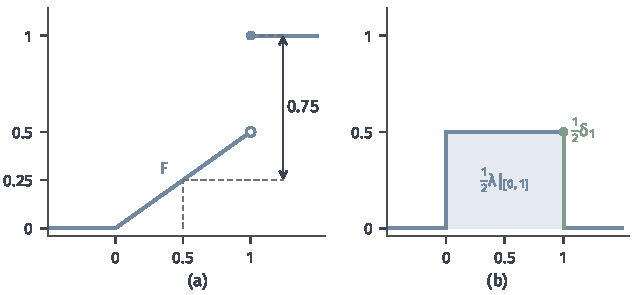
\includegraphics[width=108.000mm]{figures/04-spaces-measures-and-geometry/02-measure/matplotlib/meas-stieltjes-jump/figure.pdf}
  \caption{右连续单调函数$F$确定的Lebesgue--Stieltjes测度。(a)$F$在$[0,1)$上以斜率$1/2$增长，在$x=1$处跳跃$1/2$（实心点为$F(1)=1$，空心点为左极限$1/2$），竖向箭头是$(0.5,1]$的测度$0.75$；(b)$\mu_F$由总量$1/2$、均匀分布在$[0,1]$上的质量（蓝色密度$1/2$）与点质量$\frac12\delta_1$（绿色）组成。}
  \label{fig:meas-stieltjes-jump}
\end{BookInlineFigure}

\paragraph{Lebesgue测度}
取$F(x)=x$，得到$\mathcal B(\mathbb R)$上唯一满足$\lambda((a,b])=b-a$的测度$\lambda$。它没有点质量，所以开、闭、半开区间的测度都等于长度。

延拓定理的证明还给出更多信息。外测度$\lambda^*$由半开区间的可数覆盖定义，而每个半开区间$(a,b]$可以换成略长的开区间$(a,b+\varepsilon2^{-n})$，所以$\lambda^*$也等于用开区间覆盖的总长度的下确界，如图~\ref{fig:meas-outer-cover}所示。

\begin{BookInlineFigure}
  \centering
  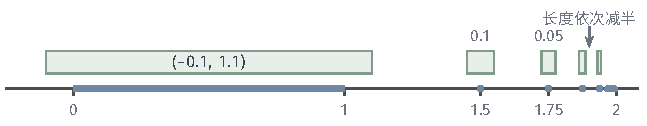
\includegraphics[width=109.552mm]{figures/04-spaces-measures-and-geometry/02-measure/tikz/meas-outer-cover/figure.pdf}
  \caption{用可数个开区间覆盖集合$E=[0,1]\cup\{1.5,1.75,1.875,\dots\}$（蓝色）。绿色区间是一种覆盖：$(-0.1,1.1)$盖住线段部分，长度依次减半的小区间盖住离散的点（只画出前几个）。这个覆盖的总长度为$1.2+0.1\cdot(1+\tfrac12+\tfrac14+\cdots)=1.4$；把各区间进一步缩短，总长度可以任意接近$1$，因此$\lambda^*(E)=1$。}
  \label{fig:meas-outer-cover}
\end{BookInlineFigure}

\begin{definition}[Lebesgue测度]
\label{def:meas-lebesgue}
关于$\lambda^*$为Carathéodory可测的全体集合称为\term{Lebesgue可测集}（Lebesgue measurable set），记作$\mathcal L$；$\lambda^*$在$\mathcal L$上的限制$\lambda$称为实轴上的\term{Lebesgue测度}（Lebesgue measure）。它在$\mathcal B(\mathbb R)$上的限制也称为Borel集上的Lebesgue测度，仍记作$\lambda$。
\end{definition}

覆盖平移后仍是覆盖，长度不变，所以$\lambda^*(E+t)=\lambda^*(E)$对一切$t\in\mathbb R$成立；判据~\eqref{eq:meas-caratheodory-criterion}中的等式随之平移，$\mathcal L$对平移封闭，Lebesgue测度具有平移不变性。

单点被$(x-\varepsilon,x+\varepsilon)$覆盖，测度为$0$，由可数次可加性，可数集的Lebesgue测度为$0$。回到有理点集：$\lambda(\mathbb Q\cap[0,1])=0$，$[0,1]$中无理数集合的测度为$1$。

同时，$[0,1]$是不可数个零测单点之并，整体测度却为$1$。这说明零测集的可数并仍零测，不可数并则不然。

\paragraph{Borel测度与它的完备化}
由Carathéodory定理，$(\mathbb R,\mathcal L,\lambda)$是完备的，且$\mathcal B(\mathbb R)\subseteq\mathcal L$。两者的差别恰好是零测集的子集，下面证明这一点。

设$E\in\mathcal L$且$\lambda(E)<+\infty$。按外测度的定义，对每个$n$有开区间列覆盖$E$且总长小于$\lambda(E)+1/n$，它们的并$U_n$是开集，$\lambda(U_n\setminus E)<1/n$。令$G=\bigcap_nU_n$，它是Borel集，满足
\[
 G\supseteq E,\qquad \lambda(G\setminus E)=0.
\]

对零测集$G\setminus E$再做一次同样的操作，得到Borel零测集$G'\supseteq G\setminus E$。于是
\[
 E=(G\setminus G')\cup(E\cap G'),
\]
第一项是Borel集，第二项包含于Borel零测集。无限测度的$E$切成可数个有限测度的片逐片处理即可。

反过来，$\mathcal L$完备且含$\mathcal B(\mathbb R)$，每个“Borel集并上Borel零测集的子集”都属于$\mathcal L$。所以$(\mathbb R,\mathcal L,\lambda)$正是$(\mathbb R,\mathcal B(\mathbb R),\lambda)$在定理~\ref{thm:meas-completion}意义下的完备化。

对一般的$F$，同样的构造给出$\mu_F$的完备化，它的可测集合族一般随$F$而变：$\mu_F=\delta_0$时，任何不含$0$的集合都是零测集的子集，完备化后全部子集都可测。所以“Borel测度”与“它的完备化”要分开说明，前者的可测范围固定为$\mathcal B(\mathbb R)$，后者的可测范围依赖测度本身。

\paragraph{Cantor集}
零测集是否一定可数？Cantor集给出否定的回答，后面它还会反复出现。

\begin{example}[Cantor集]
\label{ex:meas-cantor-set}
令$C_0=[0,1]$。把$C_{n-1}$中每个闭区间三等分，删去中间的开区间，得到$C_n$，它由$2^n$个长度为$3^{-n}$的闭区间组成，例如$C_1=[0,\tfrac13]\cup[\tfrac23,1]$。令
\[
 C=\bigcap_{n\geq0}C_n,
\]
称为\term{Cantor集}（Cantor set）。它是闭集的交，因而是闭集，也是Borel集。由$C\subseteq C_n$，
\[
 \lambda(C)\leq\lambda(C_n)=2^n\cdot3^{-n}=(2/3)^n\to0,
\]
所以$\lambda(C)=0$。

也可以从被删去的部分验算：第$n$步删去$2^{n-1}$个长度为$3^{-n}$的区间，总长度为
\[
 \sum_{n\geq1}\frac{2^{n-1}}{3^n}=\frac{1/3}{1-2/3}=1.
\]
被删去的总长度已经是$1$，留给$C$的长度只能是$0$。
\end{example}

图~\ref{fig:meas-cantor-set}画出了前四步。每一行的总长度按比例$2/3$缩小，同时区间的个数翻倍；留下的点集越来越稀，却始终非空。

\begin{BookInlineFigure}
  \centering
  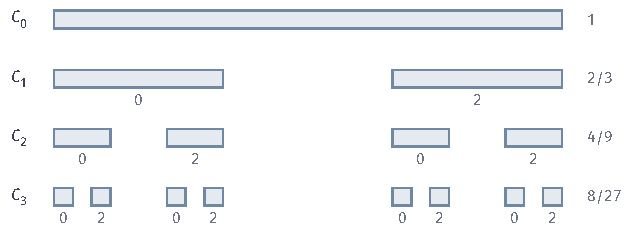
\includegraphics[width=107.142mm]{figures/04-spaces-measures-and-geometry/02-measure/tikz/meas-cantor-set/figure.pdf}
  \caption{Cantor集构造的前四步。第$n$行$C_n$由$2^n$个长度为$3^{-n}$的闭区间组成，右侧数字是总长度$(2/3)^n$；区间下方的三进制数字$0$或$2$记录这一步选择左段还是右段。}
  \label{fig:meas-cantor-set}
\end{BookInlineFigure}

Cantor集测度为零，却不可数。对每个$0$--$1$序列$s=(s_1,s_2,\dots)$，令
\[
 \phi(s)=\sum_{k\geq1}\frac{2s_k}{3^k},
\]
即三进制展开中只用数字$0$与$2$的数。前$n$位数字决定了前$n$步每一步选左段（数字$0$）还是右段（数字$2$），所以$\phi(s)\in C_n$对每个$n$成立，从而$\phi(s)\in C$。

$\phi$是单射。设$s\neq t$，第一个不同的位置为$k$，不妨$s_k=1$、$t_k=0$，则后面各项最多抵消$\sum_{j>k}2\cdot3^{-j}=3^{-k}$，于是
\[
 \phi(s)-\phi(t)\geq2\cdot3^{-k}-3^{-k}=3^{-k}>0.
\]
全体$0$--$1$序列不可数，故$C$不可数。零测性度量集合占据的长度，基数度量元素的多少，二者不能互相推出。

Cantor集还说明完备化确实增加了集合。$\lambda(C)=0$，由完备性，$C$的全部子集都Lebesgue可测，$C$与$\mathbb R$等势，所以这些子集和$\mathbb R$的全部子集一样多；而Borel集的个数只有连续统那么多，严格少于$\mathbb R$的子集个数。Borel集个数的证明要用到超限归纳，篇幅较长，读者可查阅\scite{math-folland1999real}。结论是：存在不是Borel集的Lebesgue可测集。

反过来，也存在不Lebesgue可测的集合。在$[0,1)$上规定$x\sim y$当且仅当$x-y\in\mathbb Q$，用选择公理从每个等价类选一个代表，组成集合$V$。令$\{r_k\}$为$[0,1)$中全体有理数，$V_k$为$V$按模$1$平移$r_k$的结果。这些$V_k$两两不交，并为$[0,1)$。

若$V$可测，平移不变性给出$\lambda(V_k)=\lambda(V)$，于是
\[
 1=\lambda([0,1))=\sum_k\lambda(V_k)=\sum_k\lambda(V).
\]
右边要么是$0$，要么是$+\infty$，不可能等于$1$。所以测度只能定义在某个$\sigma$代数上，不能假定全部子集都可测。

\paragraph{多维Lebesgue测度}
在$\mathbb R^d$上，把区间换成左开右闭矩形$\prod_{i=1}^d(a_i,b_i]$，长度换成体积。它们的有限不交并组成集合代数，体积在其上的可数可加性与一维相同：闭矩形是紧集，可数覆盖化为有限覆盖后，用全部矩形的边坐标把大矩形切成网格，逐块比较体积，就得到引理~\ref{lem:meas-finite-cover}的$d$维版本。

由延拓定理，得到$\mathcal B(\mathbb R^d)$上唯一满足$\lambda_d(R)=\lvert R\rvert$的测度$\lambda_d$，称为$d$维Lebesgue测度。它同样平移不变，其完备化的可测集称为$d$维Lebesgue可测集。$\lambda_d$与$d$个一维Lebesgue测度的乘积相同，这需要第~\ref{chap:integration}章的乘积测度来说明。
